%Motivation
Time series are important in many applications both in industry, e.g. in energy and finance, as well as in science, e.g. in astronomy and biology~\cite{DBLP:journals/sigmod/Palpanas15}. Therefore, efficient management and mining of time series is a task of critical importance, but also highly challenging due to the large volume and complex nature of this data. 

%Bundle/pair discovery specification
Co-evolving time series are time series that are time-aligned, i.e. they contain observation values at the same timestamps all along their duration. In this work, we focus on discovering all \textit{pairs} or \textit{groups} (called \textit{bundles}) of \textit{locally} similar co-evolving time series and extracting the \textit{subsequences} where this local similarity occurs. We consider two time series as \textit{locally similar} if the pairwise distance of their values per timestamp is at most $\epsilon$ for a time interval that lasts at least $\delta$ \textit{consecutive} timestamps.

Several research efforts have focused on similarity search over time series to detect patterns within a single or across a set of time series \cite{rakthanmanon2012searching, yeh2016matrix, linardi2018scalable, DBLP:conf/sofsem/Palpanas16}. However, to the best of our knowledge, the problem of discovering pairs or groups of similar \textit{time-aligned subsequences} within a set of \textit{co-evolving} time series has been overlooked.
%{\bf ??? describe a motivating example (even better, two examples), if we need space make all algorithms font size small, or footprint ???}
%\checknote{Does this paragraph provide some motivation?}

Discovering such pairs and bundles is useful in various applications. For instance, public utility companies employ smart meters to collect time series measuring consumption per household (e.g., for water or electricity). Identifying such bundles of time series (i.e., a number of similar subsequences over certain time intervals) can reveal similar patterns of consumption among users, allowing for more personalized billing schemes. In finance, examining time series of stock prices can identify pairs or bundles of stocks trending similarly at competitive prices over some trading period, hence offering precious insight for possible future investments.

%\checknote{Insert something similar to Figure~\ref{fig:bundles_water} and offer some intuition about the detected results.}

\begin{figure}[b]
    \centering
    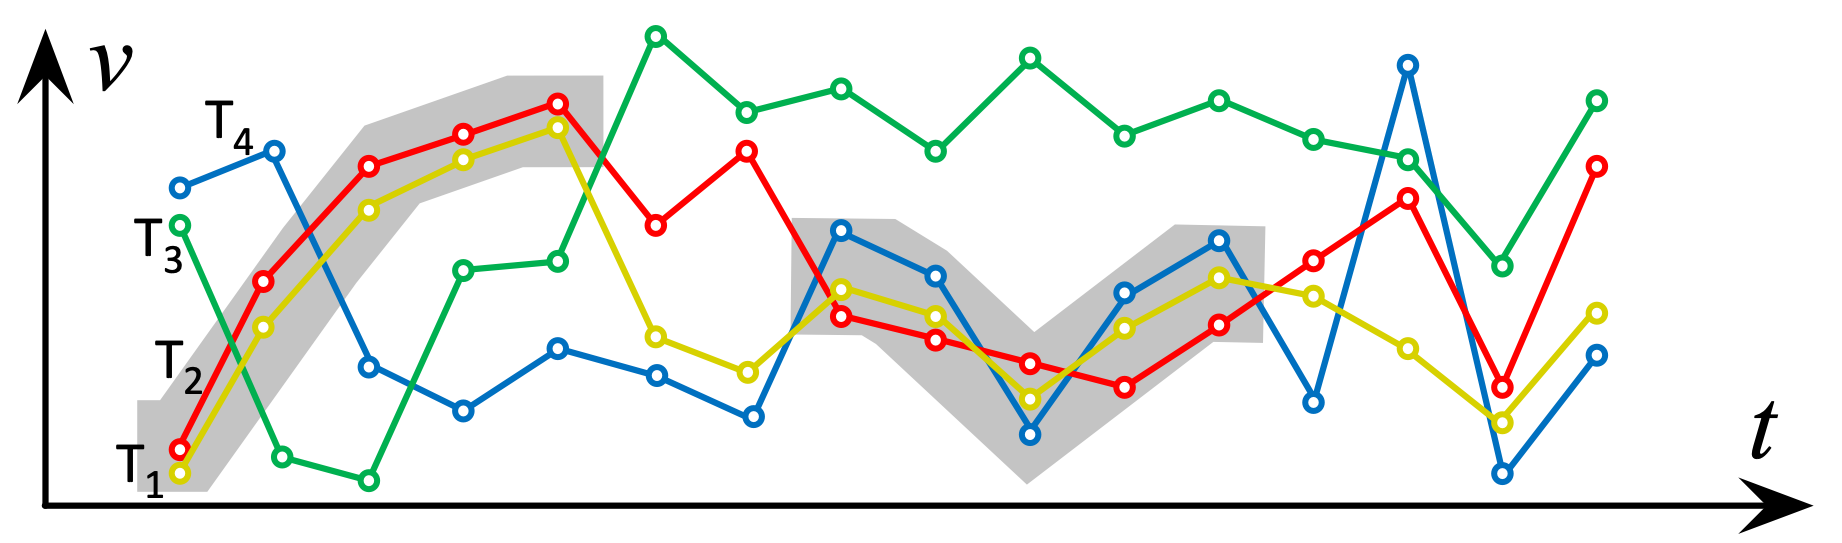
\includegraphics[width=\columnwidth]{figures/pair_flock_ex.png}
    \caption{A pair and a bundle of locally similar time series.}
    \label{fig:pair_flock_ex}
\end{figure}

Figure~\ref{fig:pair_flock_ex} illustrates an example comprising four time series depicted with different colors. We observe that from timestamp 1 to 5 the values of $T_1$ and $T_2$ are very close to each other, thus forming a locally similar pair. Similarly, from timestamp 8 to 12, the values of $T_1$, $T_2$ and $T_4$ are close to each other, forming a bundle with three members. Note that values in each qualifying subsequence may fluctuate along a bundle as long as they remain close to the respective values per timestamp of the other members in that bundle.

A real-world example is depicted in Figure~\ref{fig:water_real_ex}. These two time series represent per-hour average water consumption during a day of the week for two different households. We can observe that their respective values per timestamp (at granularity of hours, in this example) are very close to each other during a certain time period (hours 2-11), but are farther apart in the rest. Hence, an algorithm that measures the global similarity between two time series might not consider this pair as similar; however, the subsequences inside the gray strip are clearly pairwise similar, and might indicate an interesting pattern. Identifying such local similarities within a sufficiently long time interval is our focus in this paper.



% , having a similar consumption routine during night and morning (i.e., from 1am to 11 am). Considering a whole-sequence similarity measure (i.e., dynamic time warping, Euclidean distance) and given a rather tight similarity threshold $\epsilon$, a similarity search algorithm would not consider these time series as similar. However, one could require to obtain time series that are locally similar only during one or more consecutive timestamps such as the ones in the Figure.

\begin{figure}[tb]
    \centering
    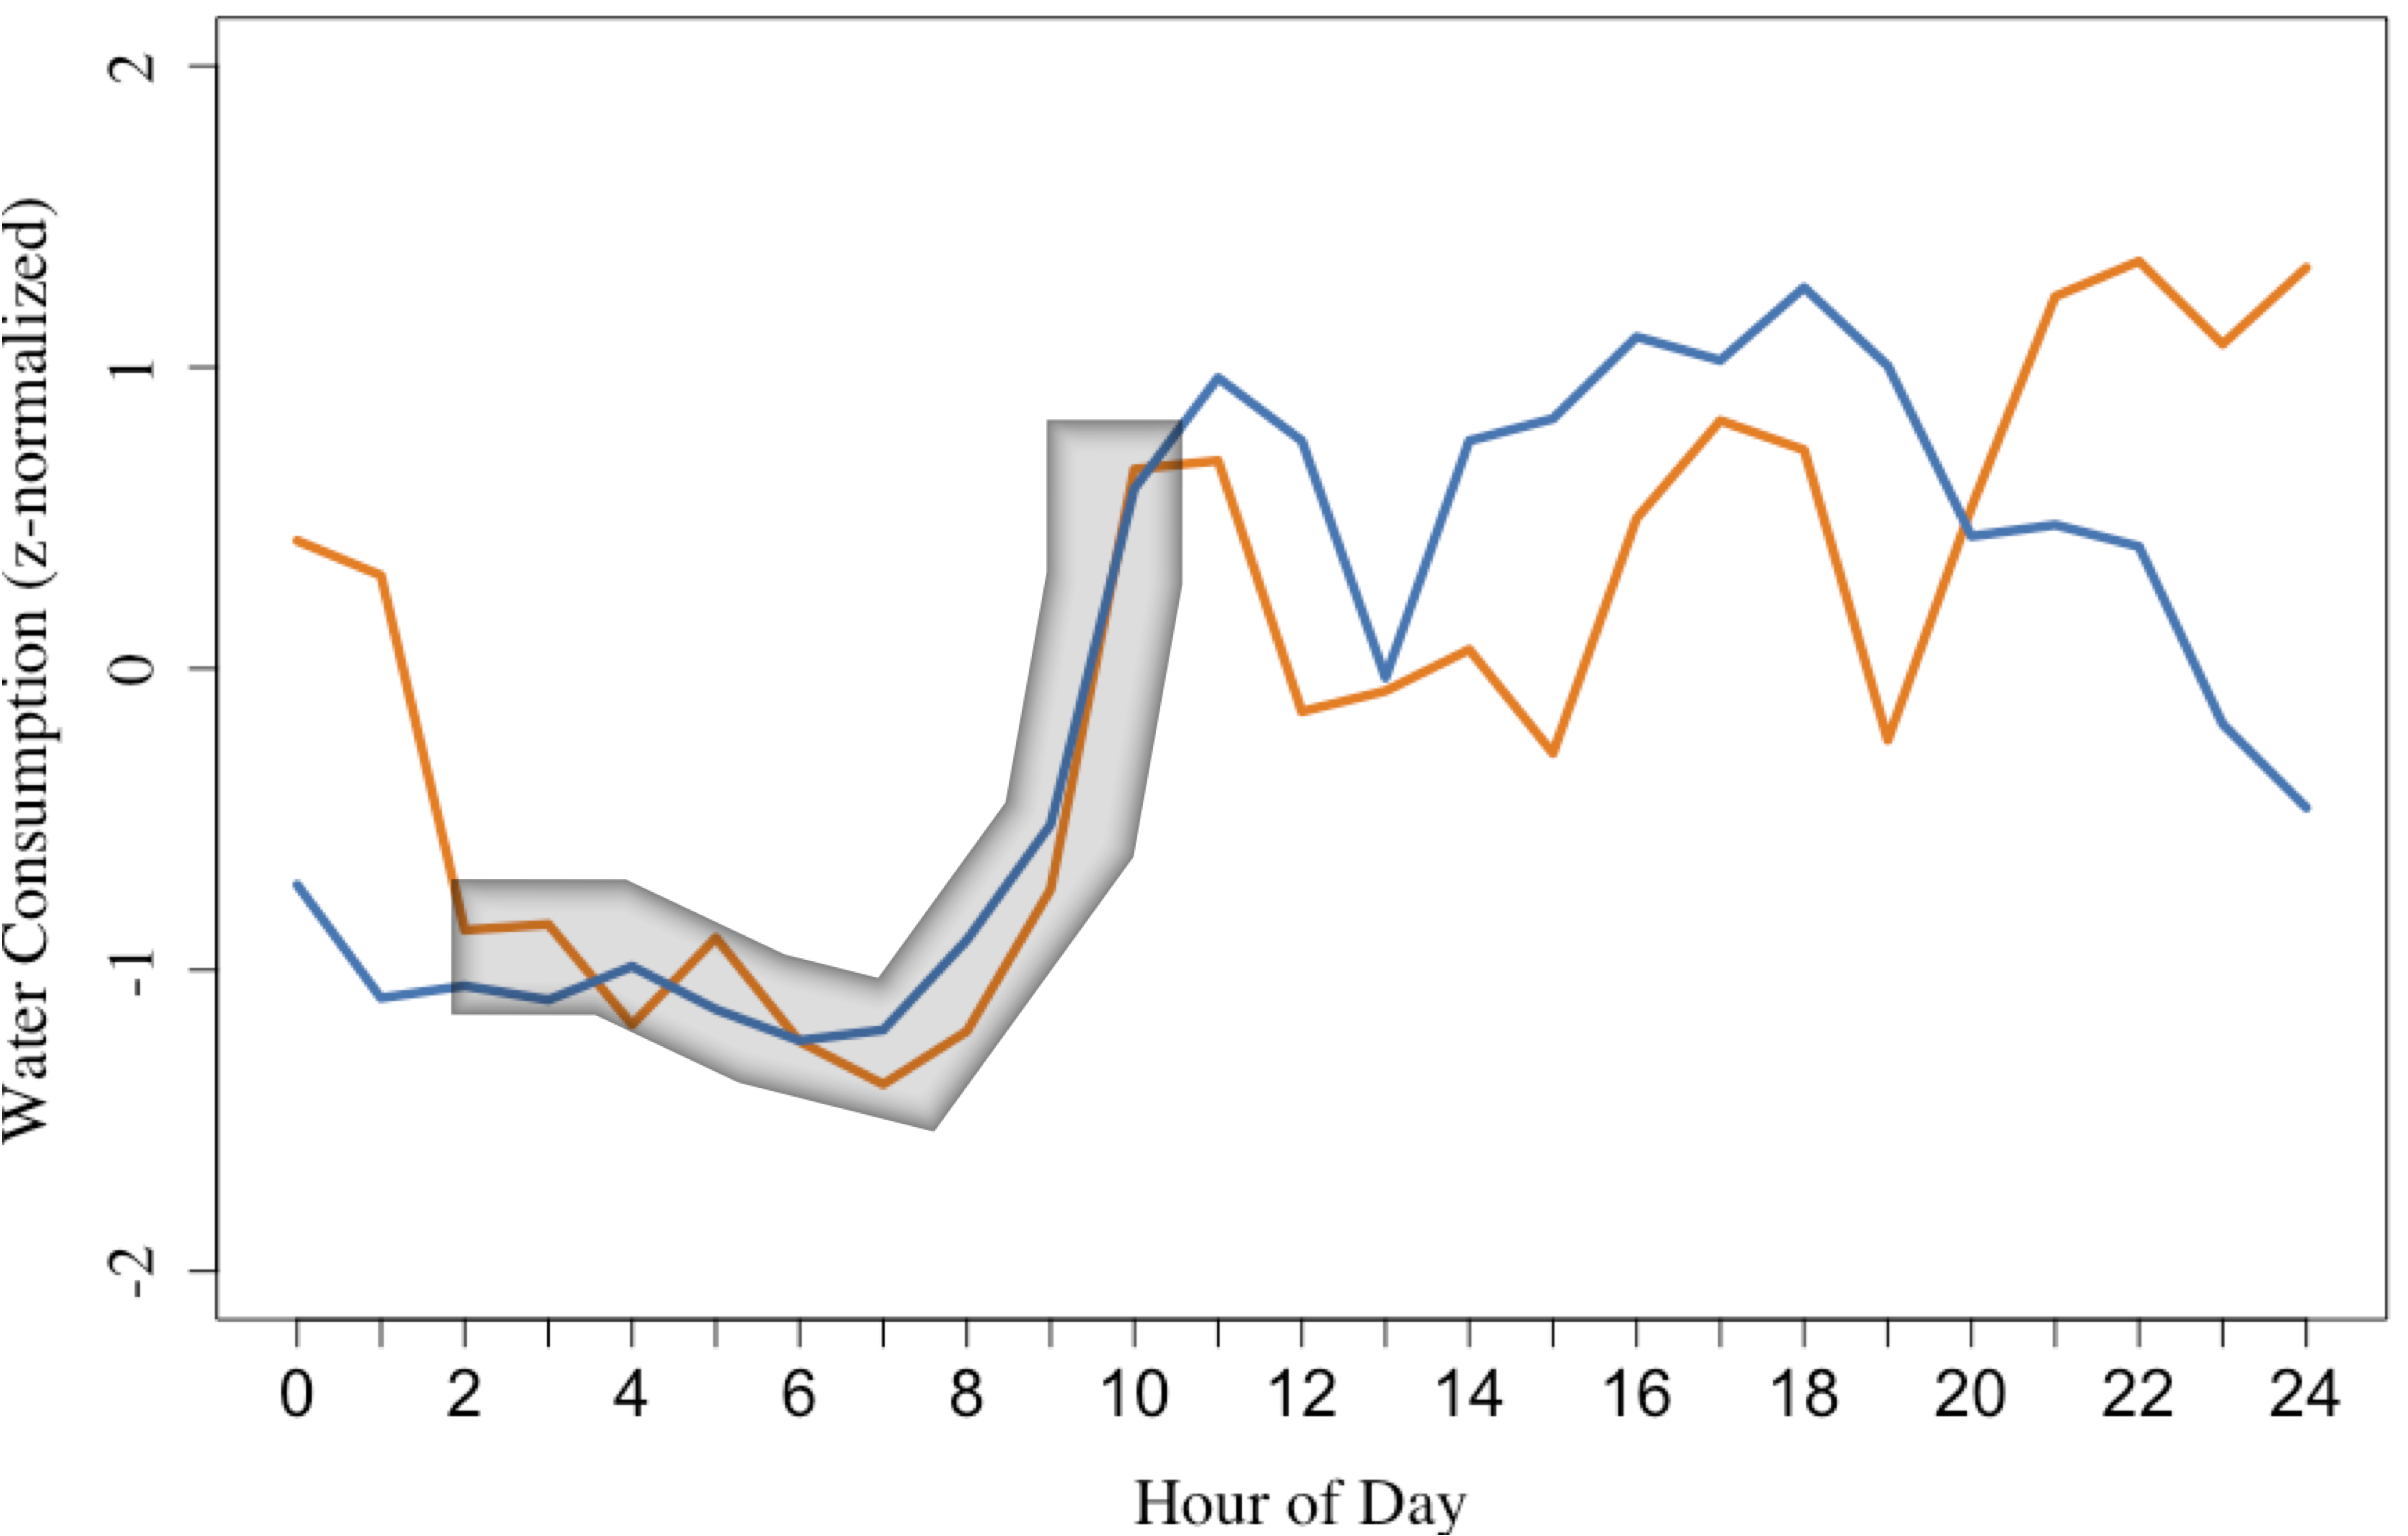
\includegraphics[width=0.9\columnwidth]{figures/water_real_ex.png}
    \caption{Pair of locally (but not globally) similar time series.} 
    \label{fig:water_real_ex}
\end{figure}


Furthermore, Figure \ref{fig:bundles_water} depicts several bundles of locally similar time series detected by our algorithms in a real-world dataset containing smart water meter measurements. The detected bundles represent different per-hour average water consumption patterns during a week. There is a wider pattern detected among 6 households during the first 30 hours of the week indicating reduced consumption (probably no permanent residence). The orange and yellow patterns indicate different morning routines during the third and fourth day of the week. The green and purple patterns represent a reduction in consumption during the late hours of the fourth and sixth day, respectively, with some intermediate consumption taking place during the night. Finally, the shorter red and light blue bundles suggest different evening patterns for two other days (respectively, decreasing and increasing consumption).

\begin{figure}[tb]
    \centering
    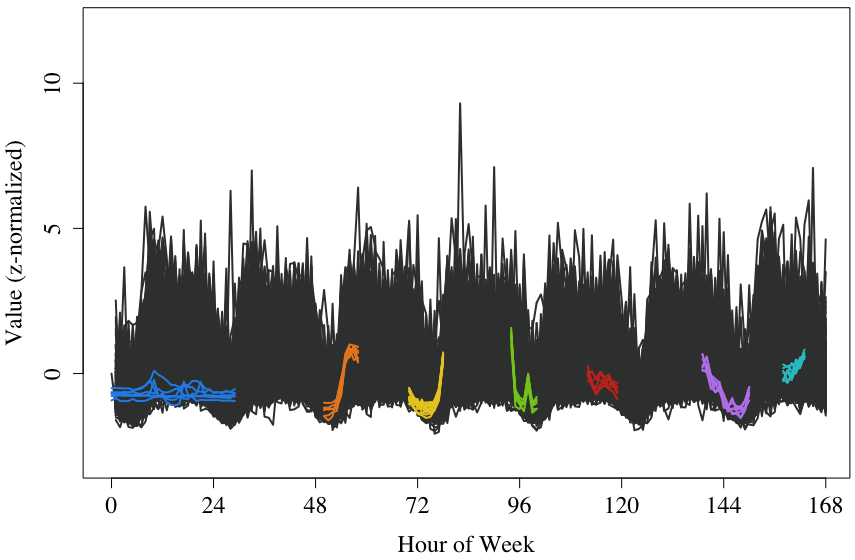
\includegraphics[width=0.85\columnwidth]{figures/bundles_water.png}
    \caption{Bundles of locally similar time series.}
    \label{fig:bundles_water}
\end{figure}

%Challenges
Discovering all possible pairs and bundles of locally similar time series, along with the corresponding subsequences, within large sets is a computationally expensive process. To find matches, a filter-verification technique can be applied. At each timestamp, the {\em filtering} step can discover candidate pairs or groups having values close to each other; then, the {\em verification} step is invoked to determine whether each such candidate satisfies the required conditions, essentially whether this match occurs throughout a sufficiently large time interval. However, both the filtering and the verification steps are expensive. The computational cost becomes especially high for the case of bundle discovery, as it has to examine all possible subsets of locally similar time series that could form a bundle. Hence, such an exhaustive search is prohibitive when the number and/or the length of the time series is large.

%General approach
In this paper, we employ a value discretization approach that divides the value axis in ranges equal to the value difference threshold $\epsilon$, in order to reduce the number of candidate pairs or bundles that need to be checked per timestamp. Leveraging this, we first propose two \textit{sweep line} scan algorithms, for pair and bundle discovery respectively, which operate according to the aforementioned filter-verification strategy. However, this process still incurs an excessive amount of comparisons, as it needs to scan all values at every timestamp. To overcome this, we introduce a more aggressive filtering  that only checks at selected \textit{checkpoints} across time, but ensuring that no false negatives ever occur. This approach incurs significant savings in computation cost, as we only need to examine candidate matches on those checkpoints only instead of all timestamps. To further reduce the number of examined candidates, we propose a strategy that judiciously places these checkpoints across the time axis in a more efficient manner. We then exploit these optimizations introducing two more efficient algorithms that significantly reduce the execution cost for both pair and bundle discovery.

%Contribution
The bundle discovery problem we address in this paper resembles the problem of \textit{flock discovery in moving objects}, where the goal is to identify sufficiently large groups of objects that move close to each other over a sufficiently long period of time \cite{gudmundsson2006computing, benkert2008reporting, vieira2009line, tanaka2015efficient}. In fact, the baseline algorithm we describe can be viewed as an adaptation of the algorithm presented  in \cite{vieira2009line}. However, to the best of our knowledge, ours is the first work to address the problems of locally similar pair and bundle discovery over co-evolving time series. Our main contributions can be summarized as follows:

\begin{itemize} 
 \item We introduce the problems of local pair and bundle discovery over co-evolving time series.
 \item We suggest an aggressive checkpoint-based pruning method that drastically reduces the candidate pairs and bundles that need to be verified, significantly improving performance.
 \item We conduct an extensive experimental evaluation using both real-world and synthetic time series, showing that our algorithms outperform the respective sweep line baselines.
\end{itemize}

%Roadmap
The remainder of this paper is organized as follows. Section \ref{sec:related} reviews related work. Section \ref{sec:problem} describes the problems. Sections \ref{sec:local_join} and \ref{sec:bundle_disc} introduce our algorithms for pair and bundle discovery, respectively. Section \ref{sec:eval} reports our experimental results, and finally Section \ref{sec:conclusions} concludes the paper.

%{\bf ??? remove this para if we need space, if we need more space make all algorithms font size small, or footprint ???}

%...Consider for example the three time series in Figure \ref{fig:local_vs_euclid}. While the green and red time series are similar in general and the Euclidean distance among them seems to be rather small (e.g., they could be a match in a similarity search scenario), there are four values that are located further than the rest. These values have a small contribution in the Euclidean distance, however, in a local distance scenario, we would require the time series to be closely located along all the timestamps. For example, the red and blue time series in the figure are considered locally close, as they are both located within the grey ribbon...